% ===============================================================
% Document Class ================================================
\documentclass{article}

% ===============================================================
% Graphic Packages ==============================================
\usepackage{graphicx}       % Permite a inclusão de imagens no documento.
\usepackage{tocloft} % Pacote para customização de listas de conteúdos, figuras e tabelas
\usepackage{tikz}           % Ferramenta poderosa para criar gráficos programaticamente dentro do LaTeX.
\usetikzlibrary{calc}       % Extensão da biblioteca TikZ que permite cálculos mais complexos de coordenadas.
\usepackage[portuguese]{babel}
\usepackage{tocloft} % Pacote para customização de listas
\renewcommand{\listfigurename}{Lista de Figuras} % Altera o título para português
\AtBeginDocument{\renewcommand{\contentsname}{Sumário}} % Altera nome de conteudo para sumário
% ===============================================================
% Mathematical Tools ============================================
\usepackage{amsmath}        % Melhora a aparência e a flexibilidade de comandos matemáticos.
\usepackage{siunitx}        % Facilita o uso de unidades do Sistema Internacional e ajuda a formatar números complexos.

% ===============================================================
% Font and Text Appearance ======================================
\usepackage{mathptmx}       % Altera a fonte padrão do documento para Times New Roman.

% ===============================================================
% Table of Contents Customization ===============================
\usepackage{tocloft}  % Oferece controle total sobre a aparência das listas de conteúdos, figuras, tabelas, etc.

% ===============================================================
% Figure Positioning ============================================
\usepackage{float}     % Melhora a interface para definir o posicionamento de objetos flutuantes como figuras e tabelas.

% ===============================================================
% Paragraph Spacing and Indentation =============================
\usepackage{setspace}  % Permite o ajuste fino do espaçamento entre linhas.
\usepackage{indentfirst} % Adiciona indentação ao primeiro parágrafo de cada seção.

% ===============================================================
% Page Layout ===================================================
\usepackage[a4paper, top=3cm, bottom=2cm, left=3cm, right=2cm]{geometry}  % Define as margens de todo o documento.
\setlength{\parindent}{4em}  % Define o tamanho da indentação para todos os parágrafos.
\setlength{\emergencystretch}{3em}

% ===============================================================
% Section Heading Customization =================================
\makeatletter
\renewcommand\paragraph{\@startsection{paragraph}{4}{\z@}%
    {2ex plus 1ex minus .2ex}%
    {1em}%
    {\normalfont\normalsize\bfseries}}
\makeatother

% ===============================================================
% Urls ==========================================================
\usepackage{hyperref} % Para criar links clicáveis
\hypersetup{
    colorlinks=true,
    linkcolor=blue,
    filecolor=magenta,
    urlcolor=blue,
    citecolor=blue,
    pdfborder={0 0 0}  % Remove o quadrado ao redor dos links
}

% ===============================================================
% Bloco de código ===============================================
\usepackage{listings}
\usepackage{xcolor}
\usepackage{courier}
\lstset{
  backgroundcolor=\color[RGB]{249,246,239},
  basicstyle=\ttfamily\footnotesize,
  breaklines=true,
  frame=single,
  numbers=left,
  numberstyle=\tiny\color{gray},
  keywordstyle=\color[RGB]{40,40,255},
  commentstyle=\color[RGB]{0,125,0},
  stringstyle=\color[RGB]{255,0,0},
  showstringspaces=false,
  rulecolor=\color{black},
  captionpos=b,
  abovecaptionskip=5pt,
  belowcaptionskip=5pt,
  xleftmargin=0.15\textwidth,
  xrightmargin=0.15\textwidth,
  morecomment=[l]{//}
}
\renewcommand{\lstlistlistingname}{Lista de Códigos} % Comando para renomear o título da Lista de Códigos

% ===============================================================
% Begin Document ================================================
\begin{document}

% ===============================================================
% Atividade 1 ===================================================
\section{Revisão da Atividade 1}

Durante a execução da Atividade 1, enfrentei um problema significativo que afetou a exatidão dos gráficos gerados. Abaixo, descrevo o erro, sua origem, a correção aplicada e a importância de revisões detalhadas no código.

\subsection{Descrição do Erro}

Nos gráficos apresentados para os casos 1 e 3 da Atividade 1, foi observado que os valores iniciais de deslocamento (\(X_0\)) não correspondiam às condições iniciais especificadas. Por exemplo, no Caso 1, onde a condição inicial de deslocamento deveria ser \(X_0 = 0\), o gráfico mostrava um valor diferente. Este erro se repetiu nos Casos 1 e 3, enquanto o Caso 2 foi simulado corretamente.

\subsection{Causa do Erro}

O erro originou-se de uma confusão na ordem das condições iniciais listadas no código de simulação para os Casos 1 e 3. Inicialmente, as condições iniciais foram inseridas em uma ordem incorreta, afetando somente estes casos:

\begin{lstlisting}[language=Scilab, caption=Condições iniciais incorretas]
  // Definicao das condicoes iniciais para cada caso de simulacao
condicoes_iniciais = [
  m/5, m/3; // Caso 3: posicao inicial (m) e velocidade inicial (m/s)
  m/4, 0;   // Caso 2: posicao inicial (m) e velocidade inicial (m/s)
  0, m/2;   // Caso 1: posicao inicial (m) e velocidade inicial (m/s)
];
\end{lstlisting}

\subsection{Correção do Erro}

A correção foi feita ajustando a ordem das condições iniciais para refletir corretamente as especificações de cada caso:

\begin{lstlisting}[language=Scilab, caption=Condições iniciais corrigidas]
// Definicao das condicoes iniciais para cada caso de simulacao
condicoes_iniciais = [
  0, m/2;   // Caso 1: posicao inicial (m) e velocidade inicial (m/s)
  m/4, 0;   // Caso 2: posicao inicial (m) e velocidade inicial (m/s)
  m/5, m/3; // Caso 3: posicao inicial (m) e velocidade inicial (m/s)
];
\end{lstlisting}

\subsection{Importância da Revisão e Validação}

Este incidente sublinha a importância de uma análise cuidadosa do código e dos resultados. Um erro aparentemente trivial na entrada de dados pode alterar significativamente os resultados de um estudo, destacando a necessidade de revisões e validações rigorosas durante o desenvolvimento de simulações científicas.

\subsection{Gráficos Corrigidos}

Os gráficos corrigidos agora refletem precisamente as condições iniciais estabelecidas para cada caso. Esses gráficos atualizados já estão incluídos no documento principal.

\subsubsection{Caso 1: Velocidade Inicial Elevada}
\begin{figure}[H]
    \centering
    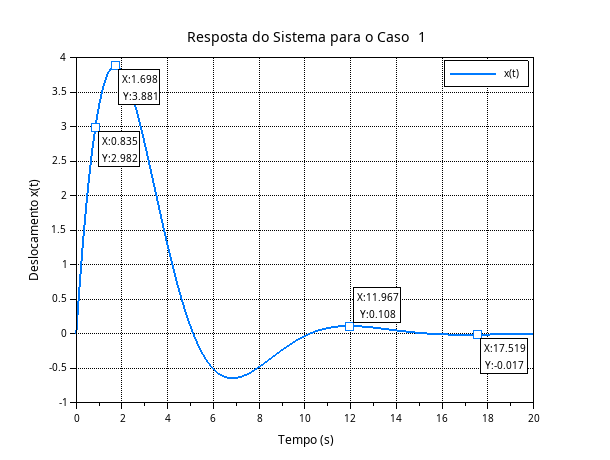
\includegraphics[width=0.6\textwidth]{atividades/1-atividade/assets/caso1.png}
    \caption{Resposta do sistema para o Caso 1}
\end{figure}
No Caso 1, o sistema é inicialmente impulsionado com uma alta velocidade (\(5 \, \text{m/s}\)), partindo do repouso (\(X_0 = 0\)). Esta condição inicial provoca uma resposta dinâmica vigorosa, onde a massa oscila com uma amplitude inicialmente elevada. O primeiro pico ocorre aproximadamente aos \(1.698 \, s\), alcançando uma altura de \(3.881 \, m\). Este pico representa a conversão máxima da energia cinética inicial em energia potencial. A subsequente queda rápida na amplitude das oscilações, como observado nos pontos seguintes, ilustra o efeito do amortecimento significativo (\(C = 7 \, \text{Ns/m}\)). Este amortecimento rapidamente reduz a amplitude das oscilações e garante que o sistema estabilize rapidamente, evitando oscilações prolongadas e retornando ao equilíbrio em aproximadamente \(17.519 \, s\), como indicado pelo deslocamento quase nulo (\(-0.017 \, m\)).

\subsubsection{Caso 2: Deslocamento Inicial Sem Velocidade}
\begin{figure}[H]
    \centering
    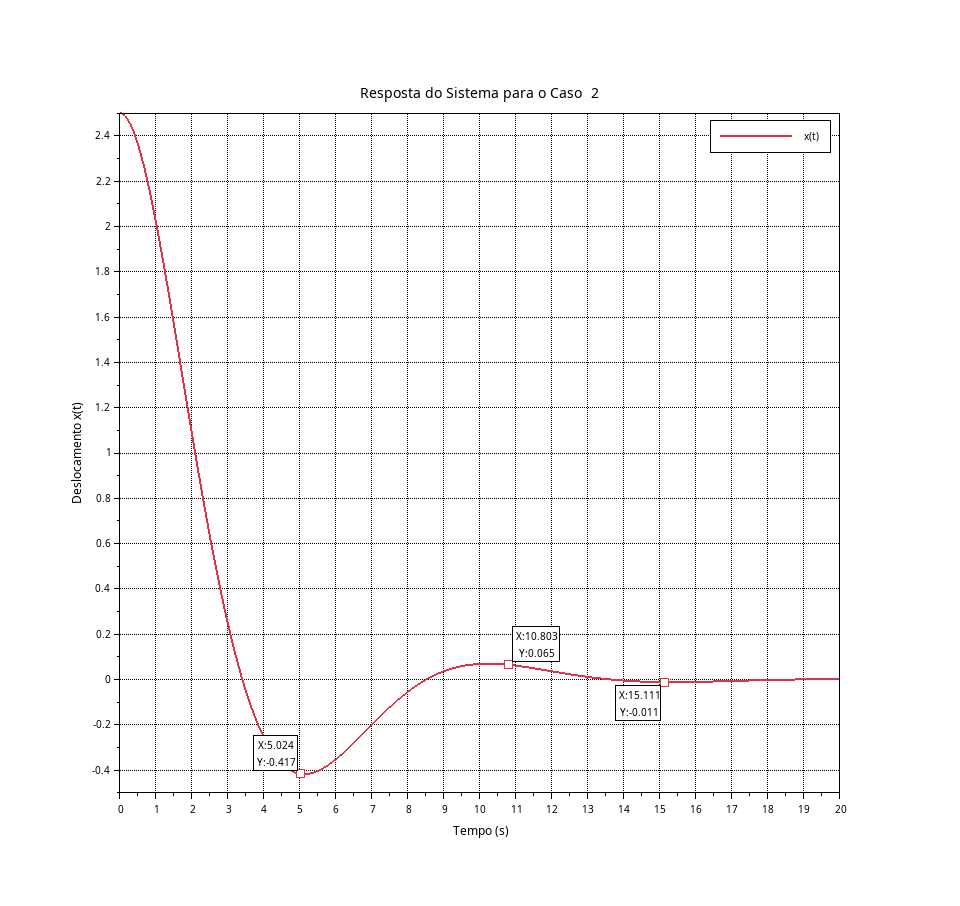
\includegraphics[width=0.6\textwidth]{atividades/1-atividade/assets/caso2.png}
    \caption{Resposta do sistema para o Caso 2}
\end{figure}
O Caso 2 é caracterizado por um deslocamento inicial de \(2.5 \, \text{m}\) sem impulso inicial de velocidade (\(V_0 = 0\)). A resposta do sistema é a de um oscilador subamortecido. Iniciando de um ponto de deslocamento máximo, o sistema mostra uma rápida resposta inicial seguida de oscilações que decaem progressivamente em amplitude. O primeiro pico de deslocamento negativo ocorre aproximadamente aos \(5.057 \, s\), com um deslocamento de \(-0.417 \, m\). Esta condição inicial destaca como a energia potencial armazenada na mola é inicialmente convertida em energia cinética, que é gradualmente dissipada pelo amortecedor. As oscilações subsequentes mostram uma diminuição gradativa na amplitude, com o sistema aproximando-se do equilíbrio em torno de \(15.026 \, s\), ilustrando uma transferência de energia mais prolongada e uma estabilização gradual em comparação ao Caso 1.

\subsubsection{Caso 3: Velocidade e Deslocamento Iniciais}
\begin{figure}[H]
    \centering
    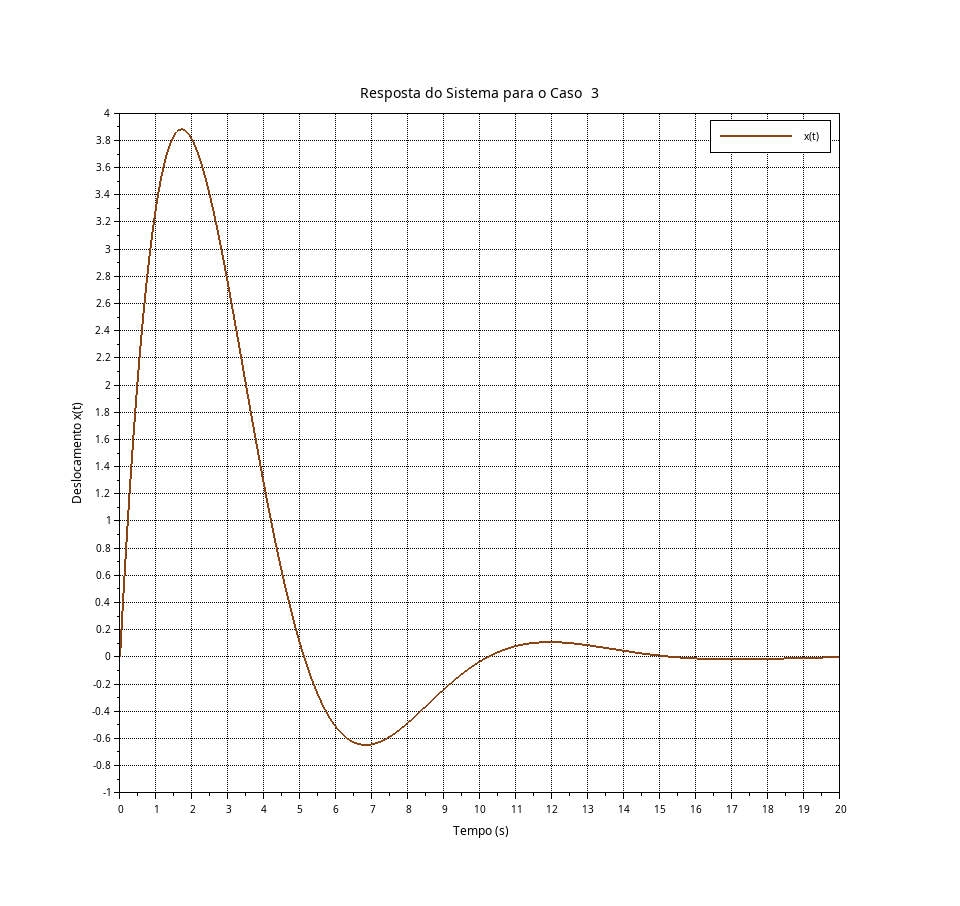
\includegraphics[width=0.6\textwidth]{atividades/1-atividade/assets/caso3.png}
    \caption{Resposta do sistema para o Caso 3}
\end{figure}
No Caso 3, o sistema inicia com condições iniciais moderadas tanto de velocidade (\(3.33 \, \text{m/s}\)) quanto de deslocamento (\(2 \, \text{m}\)). Esta configuração produz uma resposta dinâmica complexa, onde a interação entre energia cinética e potencial é claramente visível. O primeiro pico de amplitude ocorre em \(t \approx 1.241 \, s\) com um deslocamento de \(3.873 \, m\), ilustrando a conversão da energia cinética inicial em potencial. Posteriormente, as oscilações decrescem rapidamente em amplitude devido ao amortecimento significativo, estabilizando-se próximo de zero em \(t \approx 16.645 \, s\). As oscilações são mais persistentes e menos intensas do que nos outros casos, refletindo um equilíbrio dinâmico entre as energias cinética e potencial ao longo da simulação.


% ===============================================================
% Atividade 7 ===================================================
\section{Revisão da Atividade 7}

A Atividade 7 exigiu a refatoração do código Scilab utilizado para simular o Lugar Geométrico das Raízes (LGR) do sistema massa-mola-amortecedor. O objetivo era corrigir a formulação da função de transferência e aprimorar a visualização dos resultados.

\subsection{Código Original}

O código original apresentava uma formulação simplificada da função de transferência, que estava incompleta e impactava a precisão dos cálculos:

\begin{lstlisting}[language=Scilab, caption=Código Scilab para simular o Lugar geométrico das raízes original]
// Definicao dos parametros
M = 10;
C = 7;
K = 5;

// Funcao de transferencia
num = 1;
den = [M, C, K];

// Sistema
sys = syslin('c', num, den);

// Configuracao da cor para o plot do LGR
clf();
sgrid();
evans(sys, 3000, 'red');
\end{lstlisting}

\subsection{Código Refatorado}

O código foi completamente revisado para incluir uma definição detalhada da função de transferência e melhorias significativas na visualização gráfica:

\begin{lstlisting}[language=Scilab, caption=Código Scilab para simular o Lugar geométrico das raízes refatorado]
// Definicao dos parametros
M = 10;
C = 7;
K = 5;

// Funcao de transferencia
num = 1;  // Numerador e um polinomio constante
den = [M, C, K];  // Coeficientes do denominador como vetor
den_poly = poly(den, 's', 'coeff');  // Criacao do polinomio do denominador com os coeficientes

// Sistema
sys = syslin('c', num, den_poly);  // Cria o sistema com a funcao de transferencia correta

// Configuracao da figura para grafico
scf();  // Cria uma nova figura grafica
clf();  // Limpa a figura
sgrid();  // Adiciona uma grade ao grafico

// Configuracoes de visualizacao de linha
xset("line style", 4);  // Define o estilo da linha (ex: 4 - pontilhada)
xset("thickness", 3);  // Define a espessura da linha
xset("foreground", 5);  // Define a cor da linha (ex: 5 - vermelho)

// Plotando o LGR com ajustes de visualizacao
evans(sys, 50);  // Plota o LGR com 50 pontos de discretizacao

// Ajustes no grafico
xtitle("Lugar Geometrico das Raizes (LGR)", "Re(s)", "Im(s)");  // Adiciona titulo e rotulos aos eixos

// Anotacoes para polos
polos = roots(den_poly);  // Calcula os polos do sistema
for i = 1:size(polos, "r")
    // Adiciona anotacoes para cada polo no grafico
    xstring(real(polos(i)), imag(polos(i)), "Polo: "+string(polos(i)));
end

// Ajuste da visualizacao
zoom_rect([-1.8, -2.5, 0.2, 2.5]);  // Ajusta a visualizacao para incluir os polos com zoom
\end{lstlisting}

Estas alterações garantiram que a função de transferência fosse formulada corretamente, possibilitando cálculos precisos do LGR. Além disso, as melhorias visuais, como etiquetas dos polos e ajuste na escala do gráfico, permitiram uma interpretação mais clara e detalhada dos resultados, facilitando a análise da estabilidade do sistema.

\paragraph{Correlação com a Atividade 3}

Após a implementação das correções e melhorias descritas, o novo gráfico gerado pelo código refatorado agora faz mais sentido e está em consonância com os dados observados na Atividade 3. Esta consistência reforça a precisão das modificações feitas e valida a eficácia do modelo ajustado para simular o comportamento do sistema massa-mola-amortecedor. A correção do erro na formulação da função de transferência e as melhorias visuais implementadas aprimoraram a clareza dos resultados e também garantem que análises futuras sejam baseadas em dados e representações gráficas confiáveis e precisas.

A figura a seguir foi gerada após as modificações recentes no código e já foi incorporada ao relatório oficial, ilustrando o Lugar Geométrico das Raízes (LGR) do sistema massa-mola-amortecedor. Esta imagem reflete as melhorias implementadas e a precisão aprimorada na visualização dos dados.

\begin{figure}[h]
  \centering
  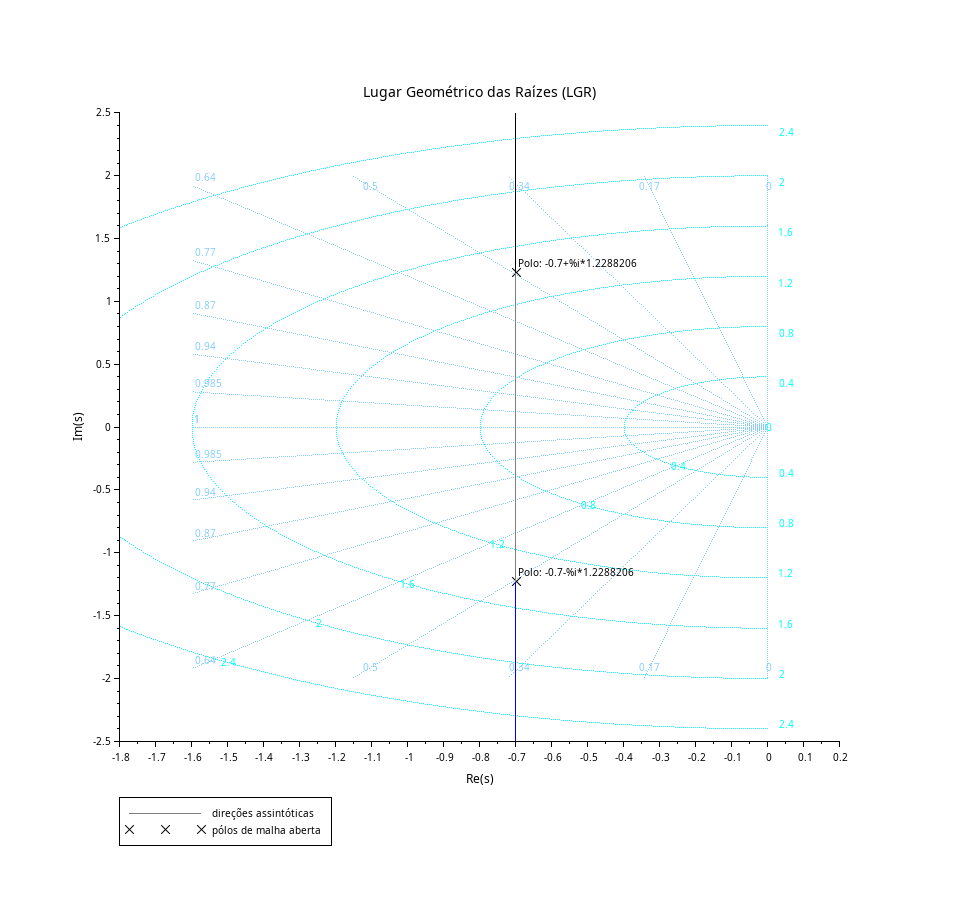
\includegraphics[width=0.8\textwidth]{atividades/7-atividade/assets/lgr.png}
  \caption{Lugar Geométrico das Raízes do sistema massa-mola-amortecedor.}
  \label{fig:LGR}
\end{figure}

% ===============================================================
% End Document ==================================================
\end{document}

